%% 11/23/2015
%%%%%%%%%%%%%%%%%%%%%%%%%%%%%%%%%%%%%%%%%%%%%%%%%%%%%%%%%%%%%%%%%%%%%%%%%%%%
% AGUJournalTemplate.tex: this template file is for articles formatted with LaTeX
%
% This file includes commands and instructions
% given in the order necessary to produce a final output that will
% satisfy AGU requirements. 
%
% You may copy this file and give it your
% article name, and enter your text.
%
%%%%%%%%%%%%%%%%%%%%%%%%%%%%%%%%%%%%%%%%%%%%%%%%%%%%%%%%%%%%%%%%%%%%%%%%%%%%
% PLEASE DO NOT USE YOUR OWN MACROS
% DO NOT USE \newcommand, \renewcommand, or \def, etc.
%
% FOR FIGURES, DO NOT USE \psfrag or \subfigure.
% DO NOT USE \psfrag or \subfigure commands.
%%%%%%%%%%%%%%%%%%%%%%%%%%%%%%%%%%%%%%%%%%%%%%%%%%%%%%%%%%%%%%%%%%%%%%%%%%%%
%
% Step 1: Set the \documentclass
%
% There are two options for article format:
%
% 1) PLEASE USE THE DRAFT OPTION TO SUBMIT YOUR PAPERS.
% The draft option produces double spaced output.
% 
% 2) numberline will give you line numbers.

%% To submit your paper:
\documentclass[draft,linenumbers]{agujournal}
\usepackage{color} % REMOVE THIS WHEN DONE!!!
\usepackage{soul} % REMOVE THIS WHEN DONE!!!
\draftfalse

%% For final version.
% \documentclass{agujournal}

% Now, type in the journal name: \journalname{<Journal Name>}

% ie, \journalname{Journal of Geophysical Research}
%% Choose from this list of Journals:
%
% JGR-Atmospheres
% JGR-Biogeosciences
% JGR-Earth Surface
% JGR-Oceans
% JGR-Planets
% JGR-Solid Earth
% JGR-Space Physics
% Global Biochemical Cycles
% Geophysical Research Letters
% Paleoceanography
% Radio Science
% Reviews of Geophysics
% Tectonics
% Space Weather
% Water Resource Research
% Geochemistry, Geophysics, Geosystems
% Journal of Advances in Modeling Earth Systems (JAMES)
% Earth's Future
% Earth and Space Science
%
%

\journalname{Geophysical Research Letters}


\begin{document}

%% ------------------------------------------------------------------------ %%
%  Title
% 
% (A title should be specific, informative, and brief. Use
% abbreviations only if they are defined in the abstract. Titles that
% start with general keywords then specific terms are optimized in
% searches)
%
%% ------------------------------------------------------------------------ %%

% Example: \title{This is a test title}

\title{Microburst Scale Size Derived from a Bouncing Packet Microburst Simultaneously Observed with the FIREBIRD-II CubeSats}

%% ------------------------------------------------------------------------ %%
%
%  AUTHORS AND AFFILIATIONS
%
%% ------------------------------------------------------------------------ %%

% Authors are individuals who have significantly contributed to the
% research and preparation of the article. Group authors are allowed, if
% each author in the group is separately identified in an appendix.)

% List authors by first name or initial followed by last name and
% separated by commas. Use \affil{} to number affiliations, and
% \thanks{} for author notes.  
% Additional author notes should be indicated with \thanks{} (for
% example, for current addresses). 

% Example: \authors{A. B. Author\affil{1}\thanks{Current address, Antartica}, B. C. Author\affil{2,3}, and D. E.
% Author\affil{3,4}\thanks{Also funded by Monsanto.}}

\authors{Mykhaylo Shumko\affil{1}, John Sample\affil{1}, Arlo Johnson\affil{1}, Bern Blake\affil{2}, Alex Crew\affil{3}, Harlan Spence\affil{4}, David Klumpar\affil{1}, Oleksiy Agapitov\affil{5}, Matthew Handley\affil{1}}

\affiliation{1}{Department of Physics, Montana State University, Bozeman, Montana, USA}
\affiliation{2}{Space Science Applications Laboratory, The Aerospace Corporation, Los Angeles, California, USA}
\affiliation{3}{The Johns Hopkins University Applied Physics Laboratory LLC, Laurel, Maryland, USA}
\affiliation{4}{Institute for the Study of Earth, Oceans, and Space, University of New Hampshire, Durham, New Hampshire, USA}
\affiliation{5}{Space Sciences Laboratory, UC Berkeley, Berkeley, California, USA}

%% Corresponding Author:
% Corresponding author mailing address and e-mail address:

% (include name and email addresses of the corresponding author.  More
% than one corresponding author is allowed in this LaTeX file and for
% publication; but only one corresponding author is allowed in our
% editorial system.)  

% Example: \correspondingauthor{First and Last Name}{email@address.edu}

\correspondingauthor{Mykhaylo Shumko}{msshumko@gmail.com}

%% Keypoints, final entry on title page.

% Example: 
% \begin{keypoints}
% \item	List up to three key points (at least one is required)
% \item	Key Points summarize the main points and conclusions of the article
% \item	Each must be 100 characters or less with no special characters or punctuation 
% \end{keypoints}

%  List up to three key points (at least one is required)
%  Key Points summarize the main points and conclusions of the article
%  Each must be 100 characters or less with no special characters or punctuation 

\begin{keypoints}
\item A bouncing packet microburst was simultaneously observed by the two FIREBIRD-II CubeSats on February 2nd, 2015.
\item The lower limit of the microburst's latitudinal and longitudinal scale sizes at LEO was $28.8 \pm 0.8$ km and $38.5 \pm 8.8$ km, respectively.
\item The microburst LEO scale sizes mapped to the magnetic equator are at least $504 \pm​ 14$ km radially, and $451 \pm 103$ km azimuthally.
\end{keypoints}

%% ------------------------------------------------------------------------ %%
%
%  ABSTRACT
%
% A good abstract will begin with a short description of the problem
% being addressed, briefly describe the new data or analyses, then
% briefly states the main conclusion(s) and how they are supported and
% uncertainties. 
%% ------------------------------------------------------------------------ %%

%% \begin{abstract} starts the second page 

\begin{abstract}
The FIREBIRD-II CubeSats simultaneously observed a bouncing packet microburst on February 2nd, 2015 during a small storm. It's latitudinal scale size is greater than $ 28.8 \pm 0.8$ km and the longitudinal scale size is greater than $38.5 \pm 8.8$ km is calculated in low earth orbit. Using the Tsyganenko 1989 magnetic field model, these scale sizes were mapped to the magnetic equator to get the radial and azimuthal scale sizes of at least $504 \pm​ 14$ km and $451 \pm 103$ km, respectively. The scale size is necessary to addreess the relative importance of microbursts in radiation belt electron losses, and to the scale sizes of whistler mode chorus waves. Lastly, the electron bounce period of the subsequent bounces was calculated and compared to analytical and numerical bounce times to validate numerous magnetic field models.
\end{abstract}

%% ------------------------------------------------------------------------ %%
%
%  TEXT
%
%% ------------------------------------------------------------------------ %%

%%% Suggested section heads:
% \section{Introduction}
% 
% The main text should start with an introduction. Except for short
% manuscripts (such as comments and replies), the text should be divided
% into sections, each with its own heading. 

% Headings should be sentence fragments and do not begin with a
% lowercase letter or number. Examples of good headings are:

% \section{Materials and Methods}
% Here is text on Materials and Methods.
%
% \subsection{A descriptive heading about methods}
% More about Methods.
% 
% \section{Data} (Or section title might be a descriptive heading about data)
% 
% \section{Results} (Or section title might be a descriptive heading about the
% results)
% 
% \section{Conclusions}

\section{Introduction}\label{Intro}
% use \citet for direct references, \citep for indirect.
The dynamics of radiation belt electrons are complex, and are driven by competition between source and loss mechanisms. A few loss mechanisms include radial diffusion \citep{Shprits04}, magnetopause shadowing \citep{Ukhorskiy06}, and pitch angle diffusion \citep{Selesnick03, Abel1998_1} due to plasma wave and Coulomb scattering. As described in \citep{Millan07, Thorne10} and references contained within, there are a variety of waves that cause pitch angle scattering, including EMIC waves, Plasmaspheric hiss, ULF waves, and whistler-mode chorus. Whistler-mode chorus predominantly occurs in the dawn sector \citep{Li09} and it accelerates (scatters) electrons with large (small) equatorial pitch angles\citep{Horne03}. It is currently believed that chorus waves are responsible for intense increases in electron precipitation flux termed microbursts. 

Historically, microbursts were first termed by \citet{Anderson1964} who used high altitude balloon observations. Few years later, \citet{Oliven1968} used the Injun 3 satelite data to reveal that chorus waves and microbursts simultaneously occir. Since then, microbursts have been observed in Low Earth Orbit (LEO) with, e.g. SAMPEX \citep{Nakamura95, Nakamura00, Blake96, Lorentzen01a, Lorentzen01b, O'Brien03, O'Brien04, Blum15} and FIREBIRD \citep{Crew16}. High altitude balloons also observe microbursts in the form of Bremsstrahlung X-rays \citep{Parks1967, Woodger15, Anderson2017}. Similar to chorus waves, microbursts predominantly occur in the dawn sector \citep{Lorentzen01b}. Understanding microburst precipitation is important to radiation belt dynamics since they have been modeled and empirically estimated to deplete the relativistic electron population of the outer radiation belt on time scales of hours to a few days \citep{O'Brien04, Thorne05, Shprits07}. 

An important parameter in the estimation of instantenous radiation belt electron losses due to microbursts is their scale size. \citet{Parks1967} used X-ray imagers on high altitude balloons to estimate the microburst scale size from Bramstrulung X-rays to be $40 \pm 14$ km. In \citet{Blake96}, a bouncing packet microburst observed with SAMPEX was estimated to have a latitudinal scale size of ``at least a few tens of kilometers", while \citet{Blake96} concluded that typically they are less than a few tens of electron gyroradii in size. \citet{Dietrich10} used SAMPEX along with ground-based VLF stations to conclude that microbursts have scale sizes less than $4$ km.

Since February 1st, 2015, microbursts have been observed by the FIREBIRD-II pair of CubeSats (FU3 and FU4) in LEO. On February 2nd, 2015, \citet{Crew16} reported a microburst with a scale size greater than 11 km. On the same day, a bouncing packet microburst was simultaneously observed on both spacecraft. The microburst decay was observed over the period of a few seconds, while the spacecraft were traversing in L. This analysis uses FU3 and FU4 to resolve the space-time ambiguity of the microburst. The rest of this paper is organized as follows: in section \ref{obs}, the spacecraft and the microburst observation will be introduced. In section \ref{analysis}, the methodology of the spacecraft time and position correction, the microburst latitudinal and longitudinal scale sizes in LEO and the magnetic equator, and electron bounce period will be explained. Lastly, in section \ref{discussion}, these results will be tied to the current empirical and theoretical understanding of microbursts and their connection to whistler-mode chorus scales.

\section{Spacecraft and Observation} \label{obs} %%%%%%%%%%%%%%%%%%%%%%%%%%%%%%%%%%%%%%%%%%%%%%%%%%%%%%%%%%%%%%%%%%%%%%%%%%
FIREBIRD-II is an identically-instrumented pair of 1.5 U CubeSats (FU3 and FU3), launched on January 31st, 2015. Their polar orbit has an apogee of 632 km and perigee of 433 km, and $99^{\circ}$ inclination \citep{Crew16}. FU3 and FU4 are flying in a leader-follower configuration with FU4 ahead, to resolve the space-time ambiguity inherent to single spacecraft missions such as SAMPEX.

Each FIREBIRD-II unit has a collimated and a surface solid state detector with complementary fields of view of $45^{\circ}$ and $180^{\circ}$. They are observing electron precipitation in six energy channels from $\sim 230$ keV to $> 1$ MeV. The adjustable sampling rate is 18.75 ms by default and can be at a fast as 12.5 ms \citep{Crew16}. 

On February 2nd, 2015 at 06:12:50 UT, a microburst with subsequent bounces was observed simultaneously on both spacecraft. Figure \ref{hires_plot} shows the electron flux data (HiRes) of the microburst. Five peaks were observed on both spacecraft. On the collimted detector, the microburst was seen up to the fourth energy channel (555 - 771 keV), while on the surface detector it was observed up to the fifth energy channel (683 - 950 keV). Only FU3 has a functioning surface detector, thus only data from the lowest four energy channels of the collimated detectors will be used for this analysis. In addition, since FU4's 5th peak in the fourth energy channel is burried in Poisson noise, only the first four peaks were used in the spatial scale analysis.

The earliest peak is not dispersed, and subsequent peaks show dispersion, which implies that this is a single microburst with subsequent decaying bounces. At this time, the spacecraft was above Sweden, latitude = $63^{\circ}$, longitude = $15^{\circ}$, altitude = 650 km, at the eastern edge of the bounce loss cone (BLC). For this analysis, the BLC is defined as the region where an electron observed at FIREBIRD's altitude will mirror at an altitude less than 100 km in the opposite hemisphere, and could be lost due to collisions in the atmosphere \citep{Abel1998_1}. For locally mirroring electrons, the mirror point in the opposite hemisphere was calculated to be 95 km using the Tsyganenko 1989 (T89) magnetic field model \citep{Tsyganenko89} with the IRBEM library. The geomagentic conditions at the time were Kp = 4, and DST = -44 nT, during the transition between the main and recovery phases. Using the spacecraft location and geomagnetic conditions, the geomagnetic location at this time was McLlwain L = 4.7, MLT = 8.3, calculated using T89. 

\begin{figure}
\includegraphics[width=\textwidth]{hires_plot_linear_8pt_smooth_err.pdf}
\caption{HiRes data of the microburst observed at February 2nd, 2015 at 06:12:50 UT, smoothed with a 150 ms window. The subsequent bounces show little energy dispersion. The energy channels' label unit is keV. As discussed in section \ref{analysis} a time correction of -2.28 s has been applied to FU3. While the flux from five energy channels is shown, only channels with reasonable counting statistics are used for the spatial scale analysis.}
\label{hires_plot}
\end{figure}

\section{Analysis} \label{analysis} %%%%%%%%%%%%%%%%%%%%%%%%%%%%%%%%%%%%%%%%%%%%%%%%%%%%%%%%%%%%%%%%%%%%%%%%%%%%%%%%%%%%%%%%%
\subsection{Time and position correction} \label{corrections}
At the beginning of the FIREBIRD-II mission, their clocks were not synchronized and there was uncertainty in their separation. The approach to calculate their relative clock difference $\delta t_{e}$, is a cross-correlation time lag analysis on temporal events that are observed simultaneously, e.g. a train of identical microbursts seen on both spacecraft on the same day as the microburst in this case study. 

Six time periods with coincident microbursts were hand-picked on February 2nd, 2015 for this analysis. The clock difference from the simultaneous microbursts were linearly fit to account for clock drift and a clock difference of $\delta t_{e} = 2.28 \pm 0.12 \ s$ was calculated. This time shift was applied to the HiRes data in Fig. \ref{hires_plot}.

To calculate their separation, the data was first corrected for the clock difference, and the same cross-correlation time lag analysis was applied on spatial events that are stationary. The observed spatial structures are believed to be stationary from similar structures observed with energies from > 35 keV to a few hundred keV on the AC-6 CubeSats while their position was confirmed with GPS \citep{Blake16}. This time lag, $\delta t_{d}$ for the spatial events is the time it takes the trailing satellite to move to the leading satellite's position.

The cross-correlation analysis on the two spatial events yields a time lag of $\delta t_{d} = 2.64 \pm 0.12$ s. Using these values, and the Two Line Elements (TLE) derived spacecraft velocity, $v = 7.57 \ km/s$ the calculated spacecraft separation was,

\begin{equation}
d = v \ \delta t_{d} = 19.9 \pm 0.9 \ km.
\end{equation}

An independent method to confirm the cross-correlation derived separation and timing difference was developed. The separation was calculated using TLEs. The TLE released for February 2nd, was anomalous and was not used. Instead, we backpropagated seven TLEs released up to five days after the microburst event, using the SGP-4 algorithm \citep{sgp4}. Then the predicted spacecraft separations at the time of the microburst event were averaged to derive a separation of $d = 18.4 \pm 1.5$ km. The timing difference was calculated using the time stamps of the FIREBIRD-II telemetry beacons during operational passes. Since they had a common time reference, the ground station computer, a time difference $\delta t_{e}  = 2.45^{+ 0.51}_{-0.98}$ s was derived. These two methods give similar results, which imply that the stationary event assumption used in the cross-correlation time lag analysis, is in fact, a reasonable assumption.

\subsection{Microburst Scale Sizes} \label{scale_size} %%%%%%%%%%%%%%%%%%%%%%%%%%%%%%%%%%%%%%%%%%%%%
Using the event and orbit topology shown in Fig. \ref{map_plot} and error propagated from the spacecraft separation, the latitudinal scale size is greater than $ 28.8 \pm 0.8$ km. This scale size is represented by the latitudinal extent of the solid and dashed boxes in Fig. \ref{map_plot}.

Since magnetospheric electrons drift eastward and were seen for multiple bounces, it is possible to calculate the longitudinal scale size of the microburst. The distance that the electrons drift azimuthally in a single bounce is given by, 

\begin{equation}
d_{az} = 2 \pi (R_E + A) \cos(\lambda) \frac{t_b}{<T_{d}>}
\label{bounce_drift}
\end{equation} where $R_E$ is the Earth's radius, $A$ is the spacecraft altitude, $\lambda$ is the magnetic latitude, $t_b$ is the electron bounce period, and $<T_{d}>$ is the electron drift period. \citet{Parks03} derived $<T_{d}>$ to be,
\begin{equation}
<T_{d}> \approx
\begin{cases}
43.8 /(L \cdot E) & \text{if } \alpha_0 = 90^{\circ} \\    62.7/(L \cdot E) & \text{if } \alpha_0 = 0^{\circ}
\end{cases}
\label{drift}
\end{equation} where E is the electron energy is MeV, L is the L shell, and $\alpha_0$ is the equatorial pitch angle. The valid limit for this analysis is $\alpha_0 = 0^{\circ}$ since electrons mirroring at FIREBIRD-II have $\alpha_0 \approx 3.7^{\circ}$. 

The microburst's longitudinal scale size is the furthest distance that its electrons drifted east and were last seen. This was calculated with $D_{az} = n \ d_{az}$ where $n$ is the number of bounces observed. Using this methodology, the longitudinal scale size is greater than $ 38.5 \pm 8.8 \ km$ for the 555 keV electrons shown as the red thin dashed box in Fig. \ref{map_plot} and greater than $ 50.8 \pm 11.4 \ km$ for the 771 keV electrons shown as the red thick dashed box in Fig. \ref{map_plot}. The stars with energy labels in Fig. \ref{map_plot} represent the locations of electrons with that energy when the microburst was seen at the first peak (P1), and drifted eastward to be last seen at P5 for FU3 and P4 for FU4.

The longitudinal and latitudinal scale sizes at LEO were mapped to the magnetic equator using the T89 magnetic field model. The radial scale size (latitudinal scale mapped from LEO) is greater than $504 \pm​ 14$ km and azimuthal scale size (longitudinal scale mapped from LEO) of 555 keV electrons is greater than $451 \pm 103$ km and of 771 keV electrons is greater than $530 \pm 119$ km.

\begin{figure}
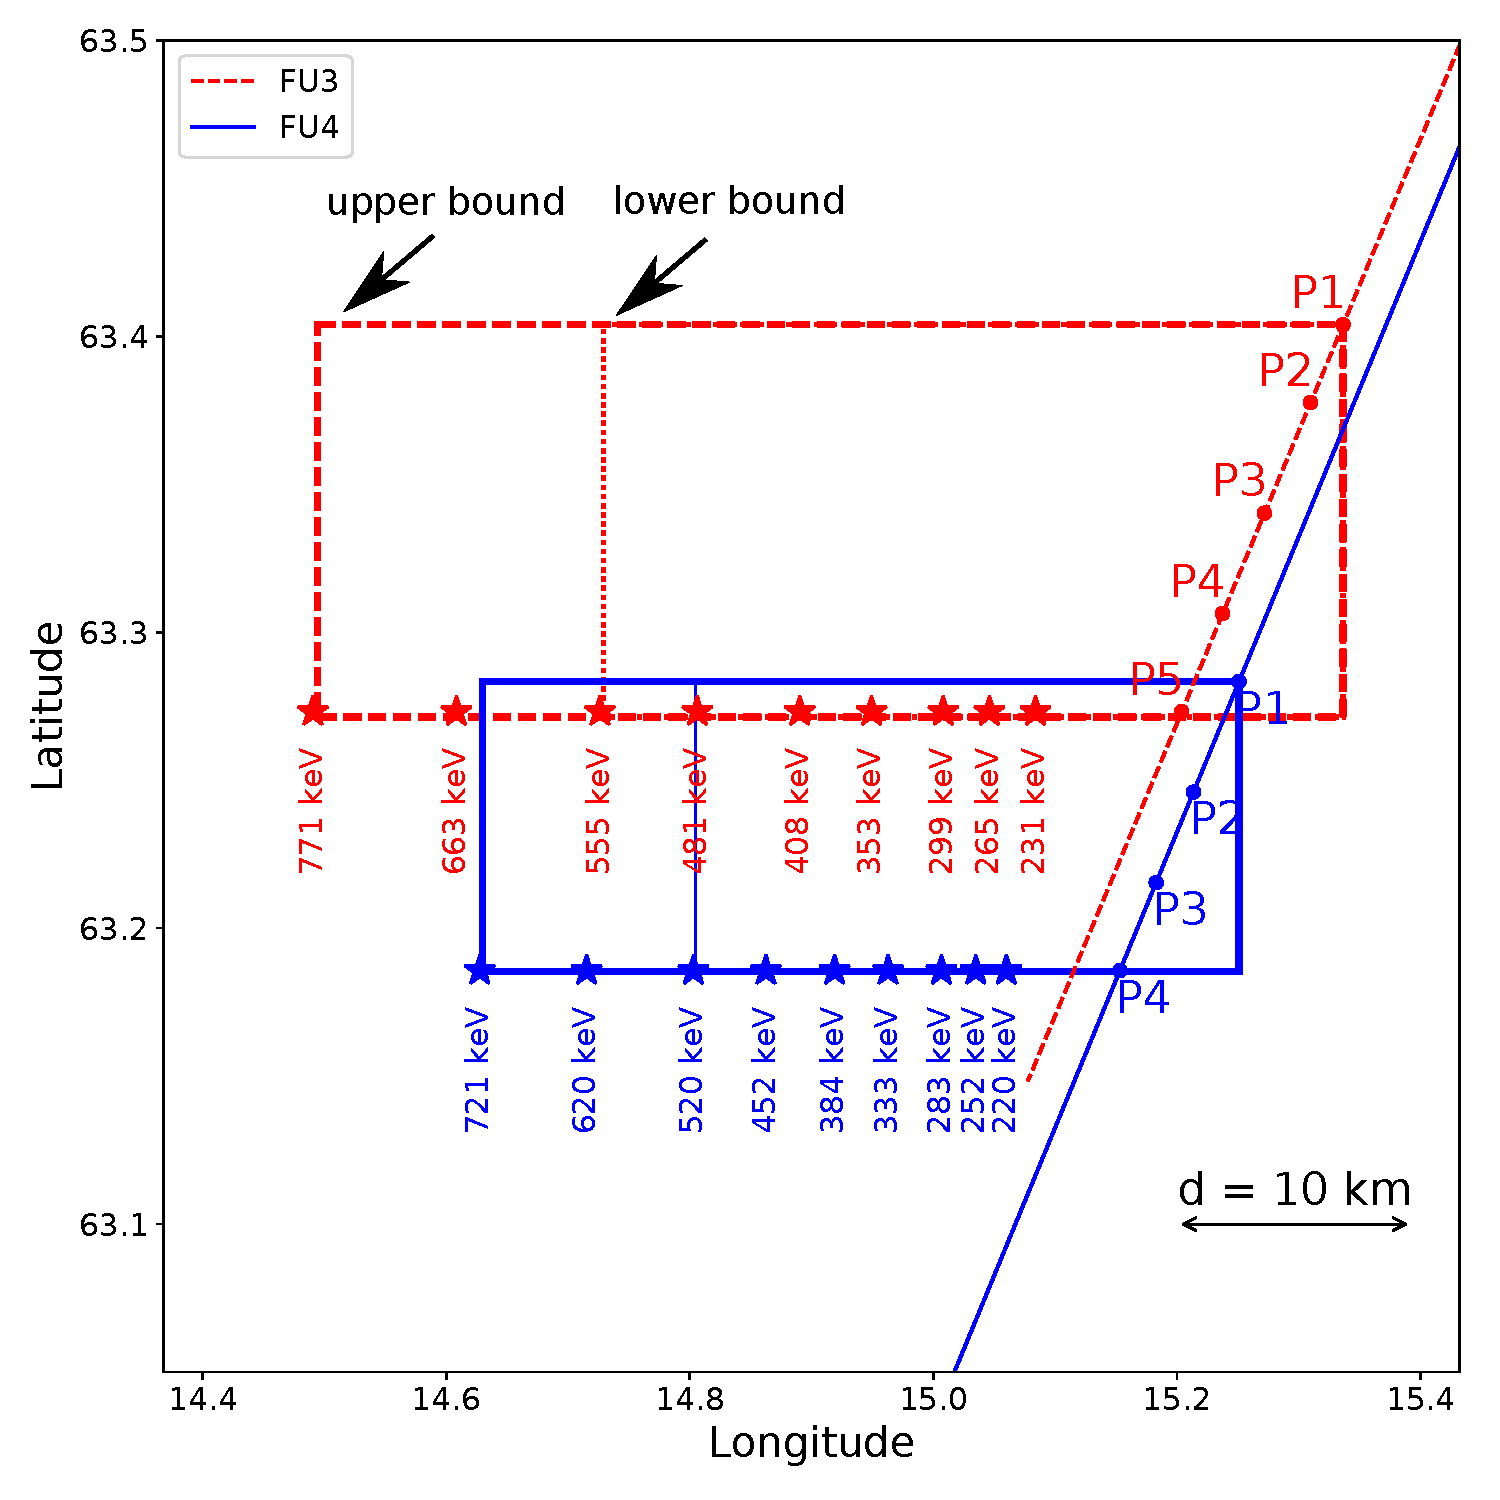
\includegraphics[width=\textwidth]{decay_microburst_distance_corrected_CH4_last_pk_drift_color.pdf}
\caption{The topology of the FIREBIRD-II orbit and the bouncing packet microburst projected onto latitude and longitude with axis scaled to equal distance. Attributes relating to FU3 shown in red dashed lines, and FU4 with blue solid lines. The spacecraft path is shown with the diagonal lines, starting at the upper right corner. The labels P(N) indicate where the spacecraft were when the N$^{th}$ peak was seen in the lowest energy channel in the HiRes data. The stars with the accompanying energy labels represent the locations of the electrons with that energy that started at time of P1, and were seen at the last peak on each spacecraft. The thick (thin) box represents the upper (lower) bound on the microburst scale size, assuming that the majority of the electrons were in the upper (lower) boundary of energy channel 4.}
\label{map_plot}
\end{figure}

\subsection{Electron Bounce Period} \label{t_b} %%%%%%%%%%%%%%%%%%%%%%%%%%%%%%%%%%%%%%%%%%%%%%%%%%%%%%%%%%%%%%%
Lastly, the observed bounce period, $t_b$ as a function of energy is calculated. To calculate the observed $t_b$ and uncertainties, the raw HiRes flux was detrended and fitted. The detrening flux (baseline) is defined in \citet{O'Brien04} as the flux at the 10th percentile over a time interval around the point to be detrended. A 0.5 s interval is used in this analysis. The flux was fitted with five Gaussians for FU3, and four for FU4. The fit uncertainty is from the detrended flux and the baseline flux summed in quadrature. Using the fit parameters, the mean $t_b$ for the lowest four energy channels was calculated and shown in Fig. \ref{tb_plot} with rectangles. 

The bounces observed with FU3 are biased to earlier times in the lowest two energy channels. This hints at the underlying distribution of electron flux within the energy channel and there are more electrons at the higher energy end of the channel. A Gaussian fit cannot account for this bias, and as a first order correction, minima between peaks was used to calculate $t_b$, and is shown in Fig. \ref{tb_plot}.

Superposed on Fig. \ref{tb_plot}, are $t_b$ curves for various models including an analytical solution from \citet{Schulz74}, and numerical models: T89, Tsyganenko 2004 (T04) \citep{Tsyganenko05}, and Olson \& Pfitzer Quiet \citep{Olson82}. The numerical $t_b$ curves were calculated using a Python wrapper for IRBEM. It traces the magnetic field line between mirror points, to calculate $t_b$ assuming conservation of energy and the first adiabatic invariant for locally mirroring electrons. 

\iffalse %%%%%%%%%%%%%%%%%%%%%%%%%%%%%%%%%%%%
The mirror point in the northern hemisphere, $m_n$ is at the FIREBIRD-II location, and $m_s$ is at the conjugate point in the southern hemisphere. Then, $t_b$ is expressed via,

\begin{equation}
t_b = 2 \int_{m_s}^{m_n}  \frac{ds}{v_{||}(E, s)}
\end{equation} where $m_n$ and $m_s$ are the northern and southern mirror points along a field line that is parameterized by $s$. The electron parallel velocity, $v_{||}(E, s)$ is calculated at each point along the field line assuming conservation of energy and the first adiabatic invariant.
\fi %%%%%%%%%%%%%%%%%%%%%%%%%%%%%%%%%%%%%%%%

\begin{figure}
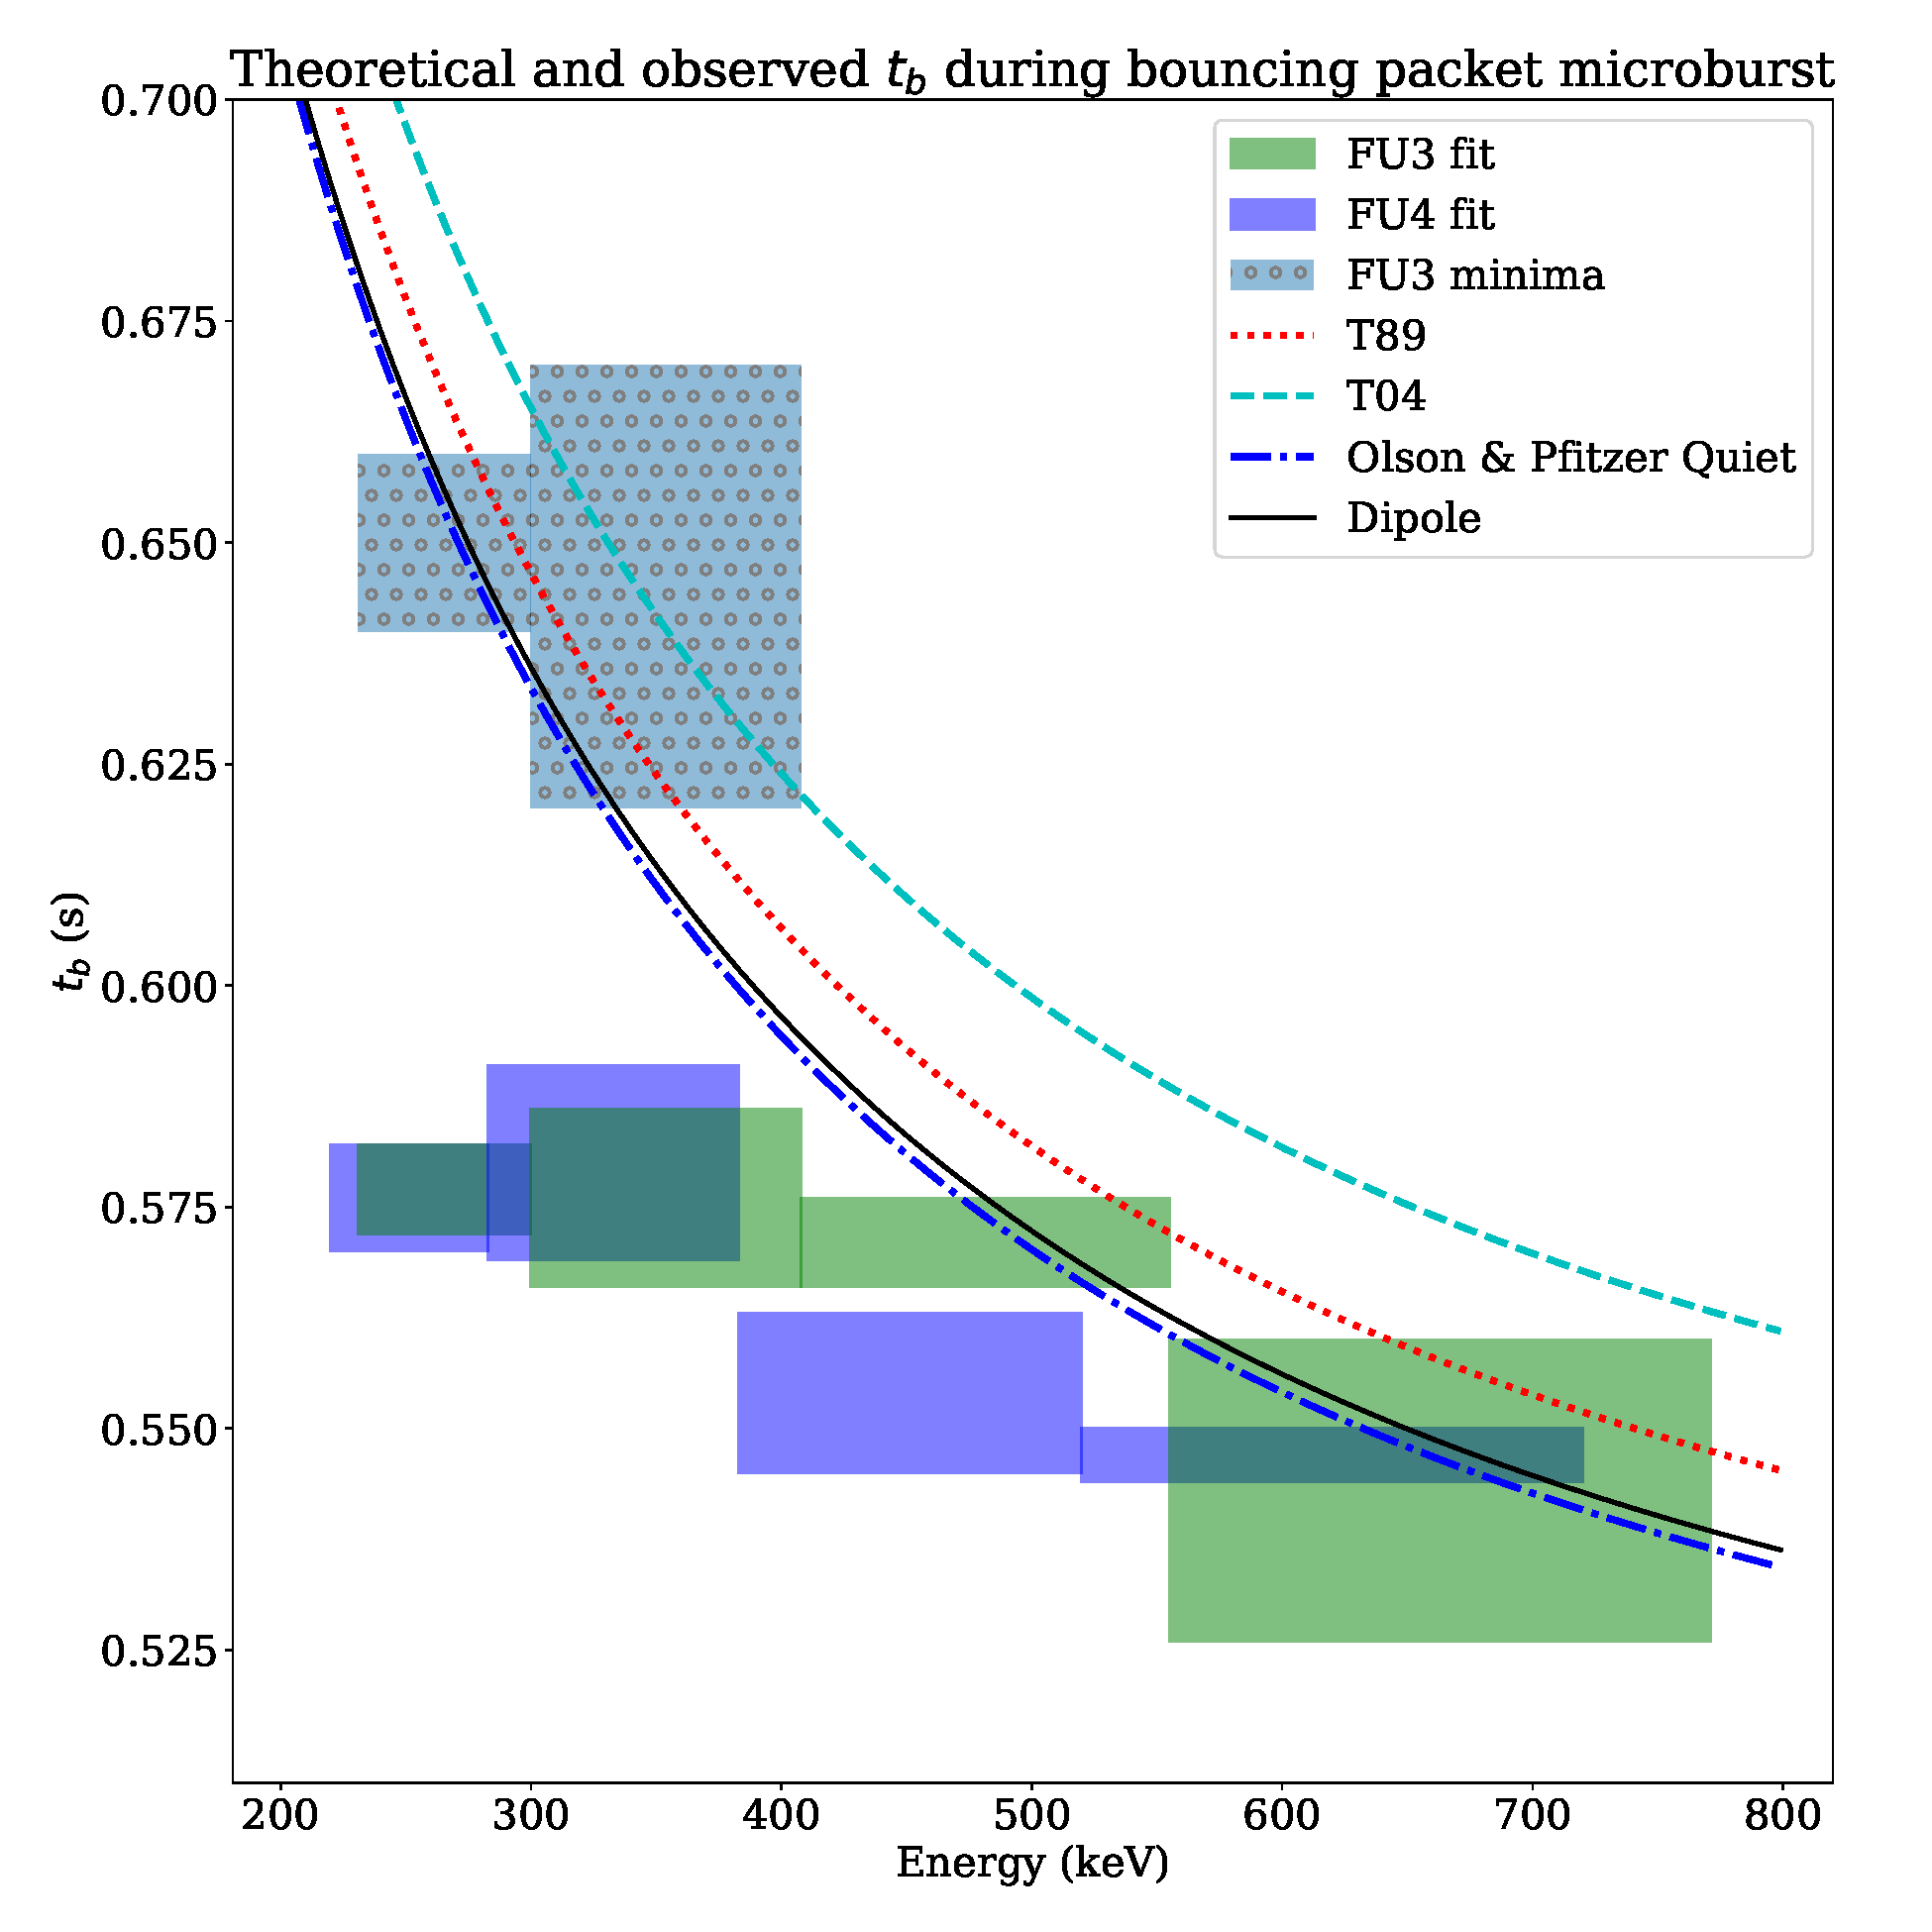
\includegraphics[width=\textwidth]{detrended_bounce_period_boxed_adj.pdf}
\caption{Observed and theoretical $t_b$ for electrons of energies from 200 to 770 keV. The solid black line is $t_b$ in a dipole magnetic field, derived in \citet{Schulz74}. The red and cyan dashed lines are the $t_b$ derived using the T89, and T04 magnetic field models with IRBEM. Lastly, the blue dashed curve is the $t_b$ derived using the Olson \& Pfitzer Quiet model. The green and purple boxes represent the observed $t_b$ for FU3 and FU4 using a Gaussian fit, respectively. The blue boxes represent the observed $t_b$ calculated with the minima between the bounces. The width of the boxes represent the width of those energy channels, and the height represents the uncertainty from the fit.}
\label{tb_plot}
\end{figure}

\section{Discussion} \label{discussion}
The scale sizes reported in section \ref{scale_size} are a lower bound. They are similar to the latitudinal scale size reported in \citet{Blake96}, and scale size reported in \citet{Parks1967}. Furthermore, the latitudinal scale size in this study is roughly $\sim 2.6$ times larger than other simultaneous microbursts reported in \citet{Crew16} and $\sim 10$ times larger than than reported in \citet{Dietrich10}.

From section \ref{scale_size}, the microburst scale size at the magnetic equator is similar to the whistler-mode chorus source scale sizes reported in \citet{Agapitov11b, Agapitov17a}. In \citet{Agapitov11b}, chorus source scale scales of $\sim 600 \ km$ were observed by CLUSTER at $L \sim 4.5$. In \citet{Agapitov17a}, The Van Allen Probes were used to measure source scale sizes of $\sim 500$ and $\sim 800$ km for upper and lower band chorus, respectively. \iffalse This mapping assumes that the interaction occurred at the magnetic equator. It is possible that the microburst electrons were scattered off the equator \citep{Lorentzen01b}, but it is outside the scope of this analysis to discern the magnetic latitude of the interaction. \fi Using the evidence from this analysis, this microburst was most likely scattered by a whistler-mode chorus.

Using the fit parameters from section \ref{t_b}, the exponential E-folding energy, $E_0$ is calculated to be $E_0 \sim 100 \ keV$. This is similar to the results in \citet{Lee05} who used STSAT-1 and \citet{Datta1997} who used a sounding rocket. It is soft for a typical microburst observed with FIREBIRD-II. Since the electron flux is falling quickly with energy, the majority of electrons seen in the fourth energy channel will be at the lower end of its energy range. Thus the lower bound of the LEO scale size (555 keV electrons), with their lower drift velocity, more realistically represents the microburst size. There is no statistically significant change in $E_0$ for subsequent bounces.

Lastly, the fitted, high energy $t_b$ shown in Fig. \ref{tb_plot} agree well to most models but T04 has the largest discrepancy at lower energies. To get an estimate of the L shell discrepancy $\Delta L$, the spacecraft position for T04 is adjusted to give better agreement with the observed $t_b$. The adjusted L shell is smaller by $\Delta L = 0.35$. On the other hand, the $t_b$ calculated using the minima in the lowest two energy channels has much better agreement.

\section{Conclusions}
The bouncing packet microburst observed by both FIREBIRD-II CubeSats shed light on the spatial and temporal properties of microbursts in LEO and the magnetic equator region. It's calculated latitudinal scale size is greater than $28.8 \pm 0.8$ km and the longitudinal scale size greater than $8.5 \pm 8.8$ km at LEO, assuming a soft energy spectra. Using the T89 magnetic field model, these scale sizes were mapped to the magnetic equator. The radial scale size is greater than $504 \pm​ 14$ km and azimuthal scale size is greater than $451 \pm 103$ km, assuming a soft energy spectra. The similarity of the derived microburst equatorial scale size to the whistler-mode chorus source region scale size, magnetospheric location, and geomagnetic conditions indicate that the microburst electrons were probably scattered by a whistler-mode chorus wave.

Lastly, the observed and theoretical bounce periods agree at high energies, but disagree by as much as $\sim 20 \%$ at the lowest energies that FIREBIRD-II observes. This is partially due to the bias to earlier times in the peaks for the two lowest energy channels, and it hints at the underlying energy-dependent electron flux in those energy channels. By using the minima method to calculate $t_b$, it is in better agreement for those energy channels. 

These rsults will be useful for future modeling efforts in areas not limited to: estimating instanteneous loss rate from the radiation belts, magnetic field modeling, and the scale sizes relationship between waves and microbursts. The scale sizes reported in this study are a lower bound, and from previous literature, it is obvious that there is a distribution of microburst scale sizes. A robust distribution cannot be derived from FIREBIRD-II, since they separated quickly in-track, and observed a small number of coincident microbursts. A follow up study is planned and a similar analysis will be applied to those microbursts, as well as to microbursts observed with the Aerocube 6 CubeSats.


%Text here ===>>>

%%

%  Numbered lines in equations:
%  To add line numbers to lines in equations,
%  \begin{linenomath*}
%  \begin{equation}
%  \end{equation}
%  \end{linenomath*}



%% Enter Figures and Tables near as possible to where they are first mentioned:
%
% DO NOT USE \psfrag or \subfigure commands.
%
% Figure captions go below the figure.
% Table titles go above tables;  other caption information
%  should be placed in last line of the table, using
% \multicolumn2l{$^a$ This is a table note.}
%
%----------------
% EXAMPLE FIGURE
%
% \begin{figure}[h]
% \centering
% when using pdflatex, use pdf file:
% \includegraphics[width=20pc]{figsamp.pdf}
%
% when using dvips, use .eps file:
% \includegraphics[width=20pc]{figsamp.eps}
%
% \caption{Short caption}
% \label{figone}
%  \end{figure}
%
% ---------------
% EXAMPLE TABLE
%
% \begin{table}
% \caption{Time of the Transition Between Phase 1 and Phase 2$^{a}$}
% \centering
% \begin{tabular}{l c}
% \hline
%  Run  & Time (min)  \\
% \hline
%   $l1$  & 260   \\
%   $l2$  & 300   \\
%   $l3$  & 340   \\
%   $h1$  & 270   \\
%   $h2$  & 250   \\
%   $h3$  & 380   \\
%   $r1$  & 370   \\
%   $r2$  & 390   \\
% \hline
% \multicolumn{2}{l}{$^{a}$Footnote text here.}
% \end{tabular}
% \end{table}

%% SIDEWAYS FIGURE and TABLE 
% AGU prefers the use of {sidewaystable} over {landscapetable} as it causes fewer problems.
%
% \begin{sidewaysfigure}
% \includegraphics[width=20pc]{figsamp}
% \caption{caption here}
% \label{newfig}
% \end{sidewaysfigure}
% 
%  \begin{sidewaystable}
%  \caption{Caption here}
% \label{tab:signif_gap_clos}
%  \begin{tabular}{ccc}
% one&two&three\\
% four&five&six
%  \end{tabular}
%  \end{sidewaystable}

%% If using numbered lines, please surround equations with \begin{linenomath*}...\end{linenomath*}
%\begin{linenomath*}
%\begin{equation}
%y|{f} \sim g(m, \sigma),
%\end{equation}
%\end{linenomath*}

%%% End of body of article

%%%%%%%%%%%%%%%%%%%%%%%%%%%%%%%%
%% Optional Appendix goes here
%
% The \appendix command resets counters and redefines section heads
%
% After typing \appendix
%
%\section{Here Is Appendix Title}
% will show
% A: Here Is Appendix Title
%
%\appendix
%\section{Here is a sample appendix}

%%%%%%%%%%%%%%%%%%%%%%%%%%%%%%%%%%%%%%%%%%%%%%%%%%%%%%%%%%%%%%%%
%
% Optional Glossary, Notation or Acronym section goes here:
%
%%%%%%%%%%%%%%  
% Glossary is only allowed in Reviews of Geophysics
%  \begin{glossary}
%  \term{Term}
%   Term Definition here
%  \term{Term}
%   Term Definition here
%  \term{Term}
%   Term Definition here
%  \end{glossary}

%
%%%%%%%%%%%%%%
% Acronyms
%   \begin{acronyms}
%   \acro{Acronym}
%   Definition here
%   \acro{EMOS}
%   Ensemble model output statistics 
%   \acro{ECMWF}
%   Centre for Medium-Range Weather Forecasts
%   \end{acronyms}

%
%%%%%%%%%%%%%%
% Notation 
%   \begin{notation}
%   \notation{$a+b$} Notation Definition here
%   \notation{$e=mc^2$} 
%   Equation in German-born physicist Albert Einstein's theory of special
%  relativity that showed that the increased relativistic mass ($m$) of a
%  body comes from the energy of motion of the body—that is, its kinetic
%  energy ($E$)—divided by the speed of light squared ($c^2$).
%   \end{notation}




%%%%%%%%%%%%%%%%%%%%%%%%%%%%%%%%%%%%%%%%%%%%%%%%%%%%%%%%%%%%%%%%
%
%  ACKNOWLEDGMENTS
%
% The acknowledgments must list:
%
% •	All funding sources related to this work from all authors
%
% •	Any real or perceived financial conflicts of interests for any
%	author
%
% •	Other affiliations for any author that may be perceived as
% 	having a conflict of interest with respect to the results of this
% 	paper.
%
% •	A statement that indicates to the reader where the data
% 	supporting the conclusions can be obtained (for example, in the
% 	references, tables, supporting information, and other databases).
%
% It is also the appropriate place to thank colleagues and other contributors. 
% AGU does not normally allow dedications.


\acknowledgments
I acknowledge the FIREBIRD team, and the members of the Space Sciences and Engineering Laboratory at MSU for their hard work to make this mission a success. In addition, I acknowledge Drew Turner for his suggestions regarding the bounce period calculations. This material is based upon work at Montana State University supported by the National Science Foundation under Grant Numbers 0838034 and 1339414.


%% ------------------------------------------------------------------------ %%
%% Citations

% Please use ONLY \citet and \citep for reference citations.
% DO NOT use other cite commands (e.g., \cite, \citeyear, \nocite, \citealp, etc.).


%% Example \citet and \citep:
%  ...as shown by \citet{Boug10}, \citet{Buiz07}, \citet{Fra10},
%  \citet{Ghel00}, and \citet{Leit74}. 

%  ...as shown by \citep{Boug10}, \citep{Buiz07}, \citep{Fra10},
%  \citep{Ghel00, Leit74}. 

%  ...has been shown \citep [e.g.,][]{Boug10,Buiz07,Fra10}.

\bibliography{/home/mike/Dropbox/0_firebird_research/A_presentations/refs}

%%  REFERENCE LIST AND TEXT CITATIONS
%
% Either type in your references using
%
% \begin{thebibliography}{}
% \bibitem[{\textit{Kobayashi et~al.}}(2003)]{R2013} Kobayashi, T.,
% Tran, A.~H., Nishijo, H., Ono, T., and Matsumoto, G.  (2003).
% Contribution of hippocampal place cell activity to learning and
% formation of goal-directed navigation in rats. \textit{Neuroscience}
% 117, 1025--1035.
%
% \bibitem{}
% Text
% \end{thebibliography}
%
%%%%%%%%%%%%%%%%%%%%%%%%%%%%%%%%%%%%%%%%%%%%%%%
% Or, to use BibTeX:
%
% Follow these steps
%
% 1. Type in \bibliography{<name of your .bib file>} 
%    Run LaTeX on your LaTeX file.
%
% 2. Run BiBTeX on your LaTeX file.
%
% 3. Open the new .bbl file containing the reference list and
%   copy all the contents into your LaTeX file here.
%
% 4. Run LaTeX on your new file which will produce the citations.
%
% AGU does not want a .bib or a .bbl file. Please copy in the contents of your .bbl file here.


%% After you run BibTeX, Copy in the contents of the .bbl file here:


%%%%%%%%%%%%%%%%%%%%%%%%%%%%%%%%%%%%%%%%%%%%%%%%%%%%%%%%%%%%%%%%%%%%%
% Track Changes:
% To add words, \added{<word added>}
% To delete words, \deleted{<word deleted>}
% To replace words, \replace{<word to be replaced>}{<replacement word>}
% To explain why change was made: \explain{<explanation>} This will put
% a comment into the right margin.

%%%%%%%%%%%%%%%%%%%%%%%%%%%%%%%%%%%%%%%%%%%%%%%%%%%%%%%%%%%%%%%%%%%%%
% At the end of the document, use \listofchanges, which will list the
% changes and the page and line number where the change was made.

% When final version, \listofchanges will not produce anything,
% \added{<word or words>} word will be printed, \deleted{<word or words} will take away the word,
% \replaced{<delete this word>}{<replace with this word>} will print only the replacement word.
%  In the final version, \explain will not print anything.
%%%%%%%%%%%%%%%%%%%%%%%%%%%%%%%%%%%%%%%%%%%%%%%%%%%%%%%%%%%%%%%%%%%%%

%%%
\listofchanges
%%%

\end{document}

%%%%%%%%%%%%%%%%%%%%%%%%%%%%%%%%%%%%%
%% Supporting Information
%% (Optional) See AGUSuppInfoSamp.tex/pdf for requirements 
%% for Supporting Information.
%%%%%%%%%%%%%%%%%%%%%%%%%%%%%%%%%%%%%



%%%%%%%%%%%%%%%%%%%%%%%%%%%%%%%%%%%%%%%%%%%%%%%%%%%%%%%%%%%%%%%

More Information and Advice:

%% ------------------------------------------------------------------------ %%
%
%  SECTION HEADS
%
%% ------------------------------------------------------------------------ %%

% Capitalize the first letter of each word (except for
% prepositions, conjunctions, and articles that are
% three or fewer letters).

% AGU follows standard outline style; therefore, there cannot be a section 1 without
% a section 2, or a section 2.3.1 without a section 2.3.2.
% Please make sure your section numbers are balanced.
% ---------------
% Level 1 head
%
% Use the \section{} command to identify level 1 heads;
% type the appropriate head wording between the curly
% brackets, as shown below.
%
%An example:
%\section{Level 1 Head: Introduction}
%
% ---------------
% Level 2 head
%
% Use the \subsection{} command to identify level 2 heads.
%An example:
%\subsection{Level 2 Head}
%
% ---------------
% Level 3 head
%
% Use the \subsubsection{} command to identify level 3 heads
%An example:
%\subsubsection{Level 3 Head}
%
%---------------
% Level 4 head
%
% Use the \subsubsubsection{} command to identify level 3 heads
% An example:
%\subsubsubsection{Level 4 Head} An example.
%
%% ------------------------------------------------------------------------ %%
%
%  IN-TEXT LISTS
%
%% ------------------------------------------------------------------------ %%
%
% Do not use bulleted lists; enumerated lists are okay.
% \begin{enumerate}
% \item
% \item
% \item
% \end{enumerate}
%
%% ------------------------------------------------------------------------ %%
%
%  EQUATIONS
%
%% ------------------------------------------------------------------------ %%

% Single-line equations are centered.
% Equation arrays will appear left-aligned.

Math coded inside display math mode \[ ...\]
 will not be numbered, e.g.,:
 \[ x^2=y^2 + z^2\]

 Math coded inside \begin{equation} and \end{equation} will
 be automatically numbered, e.g.,:
 \begin{equation}
 x^2=y^2 + z^2
 \end{equation}


% To create multiline equations, use the
% \begin{eqnarray} and \end{eqnarray} environment
% as demonstrated below.
\begin{eqnarray}
  x_{1} & = & (x - x_{0}) \cos \Theta \nonumber \\
        && + (y - y_{0}) \sin \Theta  \nonumber \\
  y_{1} & = & -(x - x_{0}) \sin \Theta \nonumber \\
        && + (y - y_{0}) \cos \Theta.
\end{eqnarray}

%If you don't want an equation number, use the star form:
%\begin{eqnarray*}...\end{eqnarray*}

% Break each line at a sign of operation
% (+, -, etc.) if possible, with the sign of operation
% on the new line.

% Indent second and subsequent lines to align with
% the first character following the equal sign on the
% first line.

% Use an \hspace{} command to insert horizontal space
% into your equation if necessary. Place an appropriate
% unit of measure between the curly braces, e.g.
% \hspace{1in}; you may have to experiment to achieve
% the correct amount of space.


%% ------------------------------------------------------------------------ %%
%
%  EQUATION NUMBERING: COUNTER
%
%% ------------------------------------------------------------------------ %%

% You may change equation numbering by resetting
% the equation counter or by explicitly numbering
% an equation.

% To explicitly number an equation, type \eqnum{}
% (with the desired number between the brackets)
% after the \begin{equation} or \begin{eqnarray}
% command.  The \eqnum{} command will affect only
% the equation it appears with; LaTeX will number
% any equations appearing later in the manuscript
% according to the equation counter.
%

% If you have a multiline equation that needs only
% one equation number, use a \nonumber command in
% front of the double backslashes (\\) as shown in
% the multiline equation above.

% If you are using line numbers, remember to surround
% equations with \begin{linenomath*}...\end{linenomath*}

%  To add line numbers to lines in equations:
%  \begin{linenomath*}
%  \begin{equation}
%  \end{equation}
%  \end{linenomath*}



